\section{Evaluation}\label{sec:evaluation}

% --------------------- Sub Section 1 ---------------------

\begin{frame}{\secname}
	\framesubtitle{Approach}

	% Our goal was to analyze existing codebases to find instances where specialization helps
	Once identified some patterns, % code patterns used in real-world codebases to overcome the lack of specialization
	we \alert{instrumented} the compiler to analyze at \alert{HIR} level % High-level Intermediate Representation (HIR) level, because here we still have access to type and lifetime information
	any function definition.

	\bigskip
	% \pause

	For each one, we created a custom \alert{AST} % Abstract Syntax Tree
	and using novel heuristics, we grouped functions that could be potentially mutually specializable. % specializable with each other
	% For example, two functions with similar names that work on similar number of arguments

	\bigskip
	% \pause

	We then calculated the \alert{tree edit distance} % between each pair of ASTs
	using the ZSS algorithm % Zhang-Shasha from 1989, which calculates the minimum number of edit operations required to transform one tree into another
	and from that, we derived a similarity score:

	$$1 - \frac{\text{dist}}{\text{max size}}$$

	% For example, if we had a function named process_int taking an i32 parameter and another function named process_float taking an f32 parameter, and the ASTs were similar enough, we could consider them to be the specialized versions of a more generic function process<T>

\end{frame}

% --------------------- Sub Section 2 ---------------------

\begin{frame}{\secname}
	\framesubtitle{Results}

	The analysis was run twice on 65 open-source Rust codebases: % from various domains, ranging from small libraries to large applications, with some having almost 1b downloads on crates.io (Rust's package registry) and others over 70k stars on GitHub
	with a similarity threshold of \alert{90\%} and \alert{99\%} respectively.

	\bigskip
	% \pause

	\begin{center}
		\begin{columns}[c]
			\column{0.1\textwidth}

			\column{0.3\textwidth}
			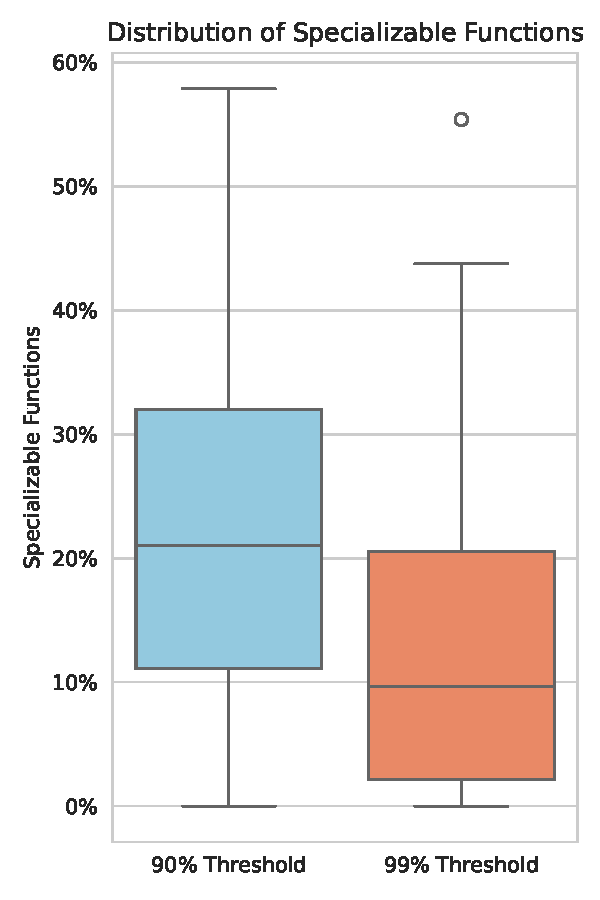
\includegraphics[width=\linewidth]{figs/specializable_functions_distribution_box_plot.pdf}
			% As we can see from the box plot on the left, the distribution of specializable functions across the analyzed codebases shows that at 90% threshold an average of more than 20% of functions could be specialized, while at 99% threshold the average drops to around 10%, which is still significant.

			\column{0.05\textwidth}

			% \pause

			\column{0.3\textwidth}
			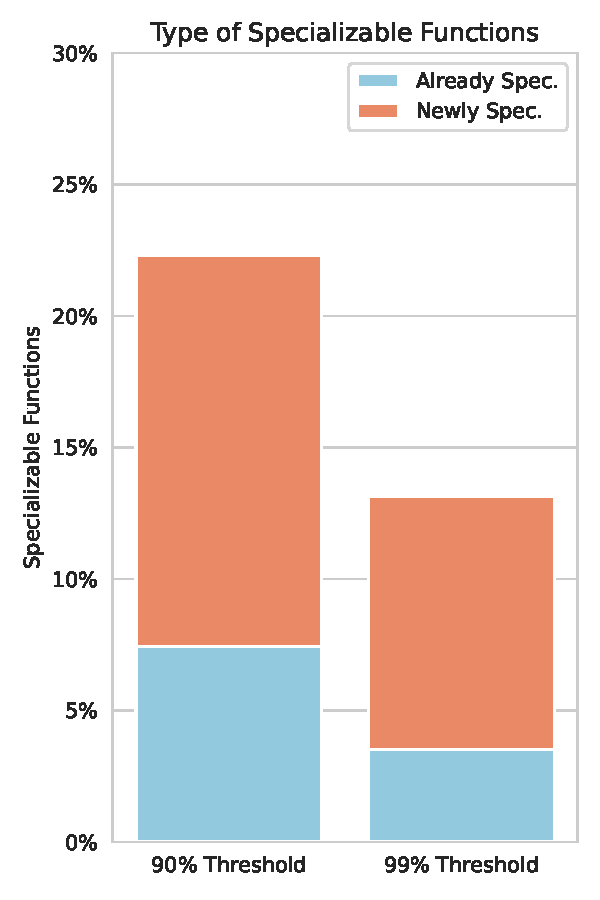
\includegraphics[width=\linewidth]{figs/specializable_functions_bar_chart.pdf}
			% The bar char on the right illustrates the proportion between functions that are already specializable using Rust's current features (in blue) and those that could benefit from additional specialization capabilities (in orange).
			% Once again we see that specialization could bring significant benefits, allowing on average to triple the number of specializable functions.

			\column{0.1\textwidth}
		\end{columns}
	\end{center}

\end{frame}

% --------------------- Sub Section 3 ---------------------

\begin{frame}{\secname}
	\framesubtitle{Results}

	We then analyzed the kinds of functions that were found to be specializable.

	\bigskip

	\begin{center}
		\begin{columns}[c]
			\column{0.6\textwidth}
			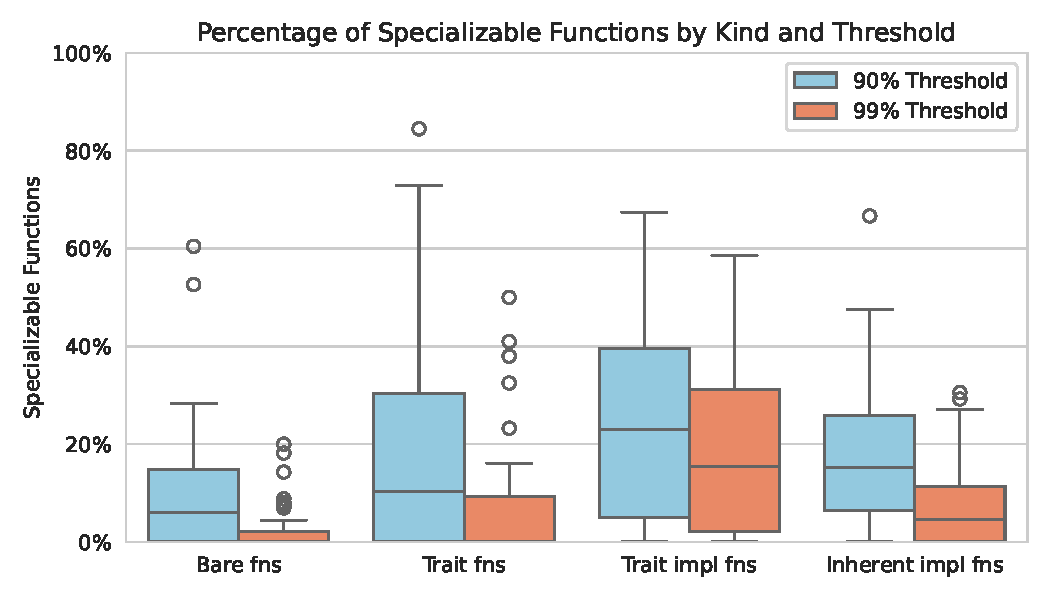
\includegraphics[width=\linewidth]{figs/specializable_functions_box_plot.pdf}
			\column{0.3\textwidth}
			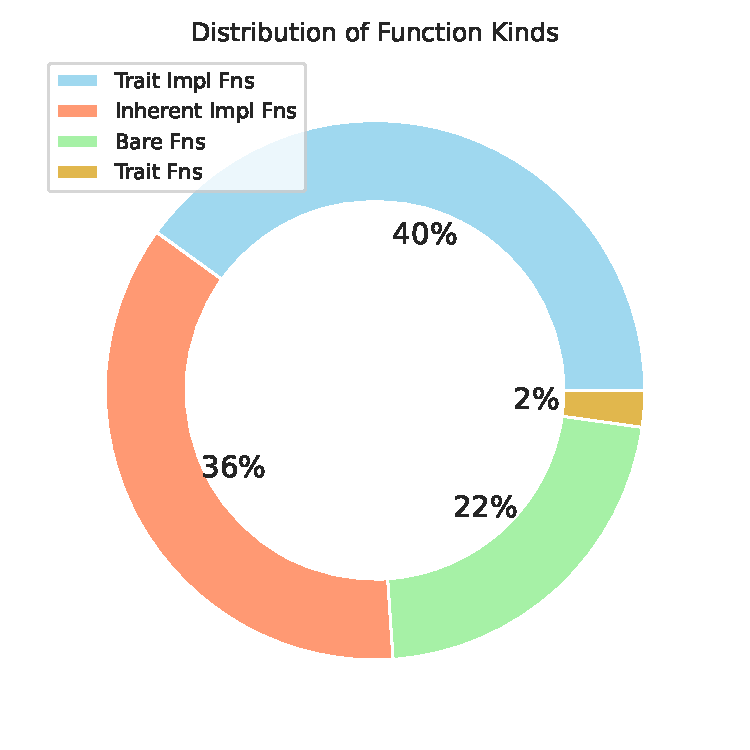
\includegraphics[width=\linewidth]{figs/functions_kind_pie.pdf}
		\end{columns}
	\end{center}
	% The box plot on the left shows the distribution of specializable functions across the analyzed codebases, grouped by function kind, while the pie chart on the right illustrates the overall proportion of specializable functions by kind.
	% As we can see, "trait impl fns" are the most common kind of functions and also the most frequently specializable.
	% This we were pretty happy about, since those "trait impl fns" are exactly the kind of functions we focused on while designing our specialization approach.

\end{frame}